\documentclass[tikz,border=2pt]{standalone}
\usepackage{amsmath}
\usetikzlibrary{arrows.meta}
\begin{document}
% Compound reversionary bonus j = 2% vested on completed anniversaries: the benefit is (1.02)^k during
% year k+1. Death at T_x = 3.4 (K_x = 3) gives benefit (1.02)^3, settled at K_x + 1 = 4, so Z = (1.02)^3 v^4.
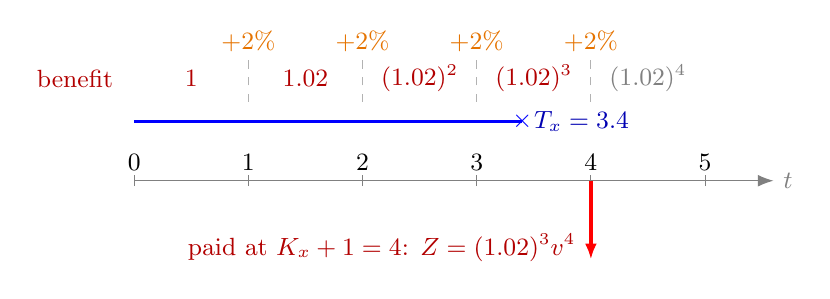
\begin{tikzpicture}[font=\small, >={Latex[length=2mm]}, x=1.45cm]
  \draw[gray, ->] (0,0) -- (5.6,0) node[right] {$t$};
  \foreach \t in {0,...,5} {
    \draw[gray] (\t,-0.07) -- (\t,0.07);
    \node[above, inner sep=2pt] at (\t,0.05) {$\t$};
  }
  % benefit level in force during each year
  \foreach \t in {1,...,4} \draw[gray!60, thin, dashed] (\t,1.0) -- (\t,1.6);
  \node[red!70!black, anchor=east] at (-0.1,1.3) {benefit};
  \node[red!70!black] at (0.5,1.3) {$1$};
  \node[red!70!black] at (1.5,1.3) {$1.02$};
  \node[red!70!black] at (2.5,1.3) {$(1.02)^2$};
  \node[red!70!black] at (3.5,1.3) {$(1.02)^3$};
  \node[gray] at (4.5,1.3) {$(1.02)^4$};
  \foreach \t in {1,...,4} \node[orange!90!black, anchor=south, inner sep=1pt] at (\t,1.6) {$+2\%$};
  % the life
  \draw[blue, very thick] (0,0.75) -- (3.4,0.75);
  \node[blue] at (3.4,0.75) {$\times$};
  \node[blue!70!black, right, inner sep=2pt] at (3.45,0.75) {$T_x=3.4$};
  % payment at the end of the year of death
  \draw[red, very thick, ->] (4,0) -- (4,-1.0);
  \node[red!70!black, anchor=east] at (3.95,-0.85) {paid at $K_x+1=4$: $Z=(1.02)^3v^4$};
\end{tikzpicture}
\end{document}
